%%%%%%%%%%%%%%%%%%%%%%%%%%%%%%%%%%%%%%%%%
% Jacobs Landscape Poster
% LaTeX Template
% Version 1.0 (29/03/13)
%
% Created by:
% Computational Physics and Biophysics Group, Jacobs University
% https://teamwork.jacobs-university.de:8443/confluence/display/CoPandBiG/LaTeX+Poster
% 
% Further modified by:
% Nathaniel Johnston (nathaniel@njohnston.ca)
%
% This template has been downloaded from:
% http://www.LaTeXTemplates.com
%
% License:
% CC BY-NC-SA 3.0 (http://creativecommons.org/licenses/by-nc-sa/3.0/)
%
%%%%%%%%%%%%%%%%%%%%%%%%%%%%%%%%%%%%%%%%%

%----------------------------------------------------------------------------------------
%	PACKAGES AND OTHER DOCUMENT CONFIGURATIONS
%----------------------------------------------------------------------------------------

\documentclass[final]{beamer}

\usepackage[scale=1.24]{beamerposter} % Use the beamerposter package for laying out the poster

\usepackage{tikz}
\usepackage{todonotes}
\usepackage{epstopdf}
\epstopdfsetup{suffix = {}}
\usepackage{hyperref}
\usepackage{subfigure}  % Written by Steven Douglas Cochran
\usepackage{amssymb,amsmath,bm}    % From the American Mathematical Society
\usepackage{siunitx} % for units like degree, ...
\sisetup{unitsep=\cdot,binary-units=true}
\usepackage{mathtools}
\usepackage{xcolor,soul}
\usepackage{geometry}
\usetheme{confposter} % Use the confposter theme supplied with this template
\usetikzlibrary{calc}

\setbeamercolor{block title}{fg=BUred,bg=white} % Colors of the block titles
\setbeamercolor{block body}{fg=black,bg=white} % Colors of the body of blocks
\setbeamercolor{block alerted title}{fg=BUred,bg=gray!70} % Colors of the highlighted block titles
\setbeamercolor{block alerted body}{fg=black,bg=gray!10} % Colors of the body of highlighted blocks


% Many more colors are available for use in beamerthemeconfposter.sty

%-----------------------------------------------------------
% Define the column widths and overall poster size
% To set effective sepwid, onecolwid and twocolwid values, first choose how many columns you want and how much separation you want between columns
% In this template, the separation width chosen is 0.024 of the paper width and a 4-column layout
% onecolwid should therefore be (1-(# of columns+1)*sepwid)/# of columns e.g. (1-(4+1)*0.024)/4 = 0.22
% Set twocolwid to be (2*onecolwid)+sepwid = 0.464
% Set threecolwid to be (3*onecolwid)+2*sepwid = 0.708

\newlength{\sepwid}
\newlength{\onecolwid}
\newlength{\twocolwid}
\newlength{\threecolwid}
\setlength{\paperwidth}{48in} % A0 width: 46.8in
\setlength{\paperheight}{36in} % A0 height: 33.1in
\setlength{\sepwid}{0.022\paperwidth} % Separation width (white space) between columns
\setlength{\onecolwid}{0.22\paperwidth} % Width of one column
\setlength{\twocolwid}{0.464\paperwidth} % Width of two columns
\setlength{\threecolwid}{0.708\paperwidth} % Width of three columns
\setlength{\topmargin}{-0.25in} % Reduce the top margin size
\setlength{\leftmargin}{-0.25in}
\setlength{\rightmargin}{-0.25in}

%-----------------------------------------------------------

\usepackage{graphicx}  % Required for including images

\usepackage{booktabs} % Top and bottom rules for tables
%\usepackage{subfigure}

%-----------------------------------------------------------
% TITLE SECTION
%-----------------------------------------------------------

\title{Plant Modeling for an Autonomous Vehicle} % Poster title

\author{Nick Nauman, Hannah Grady, Advisor: Dr. Suruz Miah} % Author(s)


\institute{Department of Electrical and Computer Engineering, Bradley University, Peoria IL} %Institution(s)
\vskip -.5cm

%-----------------------------------------------------------
% POSTER CONTENT
%-----------------------------------------------------------

\begin{document}

\addtobeamertemplate{block end}{}{\vspace*{1ex}} % White space under blocks
\addtobeamertemplate{block alerted end}{}{\vspace*{2ex}} % White space under highlighted (alert) blocks

\setlength{\belowcaptionskip}{2ex} % White space under figures
%\setlength\belowdisplayshortskip{2ex} % White space under equations

\begin{frame}[t] % The whole poster is enclosed in one beamer frame

\begin{columns}[t]

\begin{column}{\sepwid}\end{column} % Empty spacer column

\begin{column}{\onecolwid} % The first column

%-----------------------------------------------------------
% OBJECTIVE AND CONTRIBUTION
%-----------------------------------------------------------

\begin{alertblock}{Objective and Contributions}
%
\textbf{Objective}
\vskip -0.75cm
\begin{itemize}
    \item Provide accurate plant models of each autonomous vehicle subsystem to be used for designing controllers
\end{itemize}
%\begin{itemize}
%    \item Develop a platform that allows mobile devices to control helicopters with the least amount of error via an embedded system 
%\end{itemize}
%
\vskip -1cm
\textbf{Contribution}
\vskip -0.75cm
\begin{itemize}
	\item Determine if System Identification or Neural Network modeling produces better models 
	\item Non-linearity modeling
%    \item Determine trade-offs between traditional control techniques and machine learning
    %\item Embedded System Implementation
    %\item Mobile Device Control 
    %\item Multi-Helicopter Application
\end{itemize}
\vskip -0.75cm
\textbf{Applications}
\vskip -0.75cm
\begin{itemize}
	\item Use in testing to help develop more accurate vehicle controllers
	\item Create a guide for modeling future vehicle subsystems
%    \item Teleoperation approach to search and rescue 
%    \item Aerial turbulence resistance 
\end{itemize}

%


\end{alertblock}

%-----------------------------------------------------------
% PROBLEM SETUP
%-----------------------------------------------------------
\vskip -1cm
\begin{block}{Problem Setup}
%\vskip -1cm
%\begin{enumerate}
%    \item Develop and linearize system model
%    \item Simulate algorithms in MATLAB
%    \item Test algorithms on desktop computer using USB connection 
%    \item Test algorithms on Raspberry Pi microcontroller
%    \item Test algorithms on mobile device
%\end{enumerate}


%\vskip -1cm
$\bullet$ Conducted a literature review to look for existing solutions
$\bullet$ System Architecture 
\begin{figure}
	\centering
	\begin{tikzpicture}
    \tikzstyle{every node} = [font=\footnotesize]
    \tikzstyle{block} = [draw, rectangle, fill=green!15, rounded corners=5pt, minimum width=4.5 cm, minimum height=0.75 cm]
    \tikzstyle{sum} = [draw, circle,fill=orange!15]
    % place nodes
    \node[sum](sum){$\sum$};
    \node[block,right of=sum,node distance=2 cm, text width=1.25cm,text centered](steeringController){Steering controller};
    \node[block,right of=steeringController,node distance=2.25 cm, text width=1.3cm,text centered](steeringSubsystem){Steering subsystem};

    % Connections
    \draw[stealth-,thick]
    (sum.west)--node[very near start,above]{$+$}++(-0.5,0)node[above]{$\theta^{\text{ref}}$};
    \draw[-stealth,thick]
    (sum.east)--node[midway,above]{Error}(steeringController);
    \draw[-stealth,thick]
    (steeringController.15)--node[midway,above]{$v_A$}(steeringSubsystem.165);
    \draw[-stealth,thick]
    (steeringController.-15)--node[midway,above]{$v_B$}(steeringSubsystem.-165);
    \draw[-stealth,thick]
    (steeringSubsystem.east) --coordinate (tt) ++(0.5,0)node[above]{$\theta(t)$};
    \fill
    ($(steeringSubsystem.east)+(0.25,0)$) circle [radius=2pt];
    \draw[-stealth,thick]
    (tt) -- ++(0,-0.75) -|(sum.south)node[pos=0.9,left]{$-$};
    
  \end{tikzpicture}
  % \captionsetup{justification=centering, margin=3cm}

  % 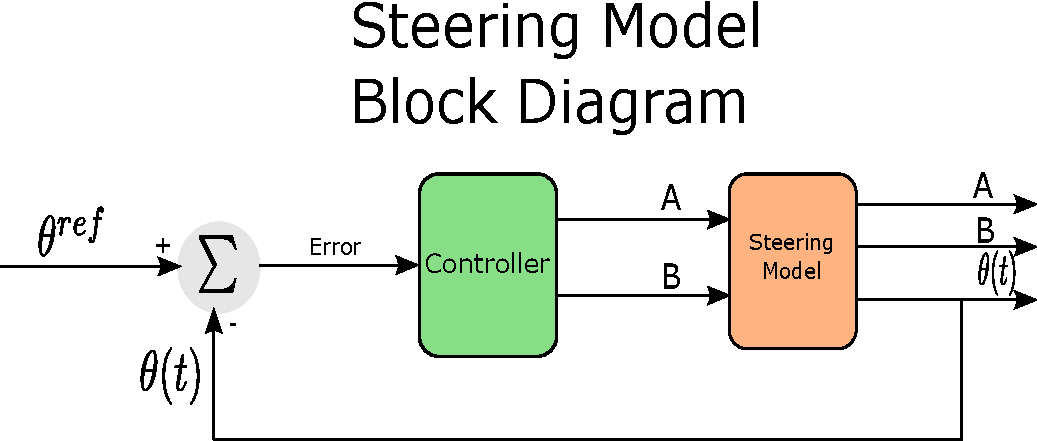
\includegraphics[width=2.5in]{figs/inkscape/steeringModelBlockDiagram}
  \caption{Steering subsystem block diagram.}
  \label{fig:steeringModelBlockDiagram}
\end{figure}


\begin{figure}
	\centering
	 \begin{tikzpicture}
    \tikzstyle{every node} = [font=\footnotesize]
    \tikzstyle{block} = [draw, rectangle, fill=green!15, rounded corners=5pt, minimum width= 5 cm, minimum height=1.5 cm]
    % place nodes
    \node[block,text width=1.75cm,text centered](accelSubsystem){Acceleration subsystem};
    % Connections
    \draw[stealth-,thick]
    (accelSubsystem.180)--node[very near end,above]{Acceleration pedal voltages}++(-5.0,0);
    \draw[-stealth,thick]
    (accelSubsystem.0)--node[very near end,above]{Acceleration pedal position}++(5.0,0);
  \end{tikzpicture}
    \caption{Acceleration subsystem block diagram}
    \label{fig:accelModelArchitecture}
\end{figure}


\begin{figure}
	\centering
	  \begin{tikzpicture}
    \tikzstyle{every node} = [font=\footnotesize]
    \tikzstyle{block} = [draw, rectangle, fill=green!15, rounded corners=5pt, minimum width=4.5 cm, minimum height=2.0 cm]
    % place nodes
    \node[block,text width=1.25cm,text centered](brakeSubsystem){Brake subsystem};

    % Connections
    \draw[stealth-,thick]
    (brakeSubsystem.140)--node[pos=0.65,above]{Pressure voltages}++(-4.5,0);
    \draw[stealth-,thick]
    (brakeSubsystem.180)--node[pos=0.65,above]{Stroke voltages}++(-4.5,0);
    \draw[stealth-,thick]
    (brakeSubsystem.-140)--node[pos=0.65,above]{On/Off switch}++(-4.5,0);
    \draw[-stealth,thick]
    (brakeSubsystem.30)--node[pos=0.5,above]{Pedal position}++(4.5,0);
    \draw[-stealth,thick]
    (brakeSubsystem.-30)--node[pos=0.5,below]{Brake pressed}++(4.5,0);
    
  \end{tikzpicture}
    % \captionsetup{justification=centering, margin=3cm}
    % \includegraphics[width=2.5in]{figs/inkscape/brakeModelArchitecture}
    \caption{Brake subsystem block diagram}
    \label{fig:brakeModelArchitecture}
\end{figure}


\begin{figure}
    \centering
        \begin{tikzpicture}
    \tikzstyle{every node} = [font=\footnotesize]
    \tikzstyle{block} = [draw, rectangle, fill=green!15, rounded corners=5pt, minimum width=4.5 cm, minimum height=1.5 cm]
    % place nodes
    \node[block,text width=1.75cm,text centered](speedControlSubsystem){Speed Control subsystem};

    % Connections
    \draw[stealth-,thick]
    (speedControlSubsystem.180)--node[very near end,above]{Desired vehicle speed}++(-4.0,0);
    \draw[-stealth,thick]
    (speedControlSubsystem.0)--node[very near end,above]{Actual vehicle speed}++(4.0,0);
    
  \end{tikzpicture}
    \caption{Speed Control subsystem block diagram}
    \label{fig:speedControlModelArchitecture}

\end{figure}


\begin{figure}
    \centering
  \begin{tikzpicture}
    \tikzstyle{every node} = [font=\footnotesize]
    \tikzstyle{block} = [draw, rectangle, fill=green!15, rounded corners=5pt, minimum width=4.5 cm, minimum height=2 cm]
    % place nodes
    \node[block,text width=1.25cm,text centered](speedSubsystem){Speed subsystem};

    % Connections
    \draw[stealth-,thick]
    (speedSubsystem.140)--node[very near end,above]{Acceleration pedal position}++(-5.0,0);
    \draw[stealth-,thick]
    (speedSubsystem.180)--node[very near end,above]{Brake pedal position}++(-5.0,0);
    \draw[stealth-,thick]
    (speedSubsystem.-140)--node[near end,above]{Shifter Gear}++(-5.0,0);
    \draw[-stealth,thick]
    (speedSubsystem.0)--node[near end,above]{Vehicle Speed}++(5.0,0);
    
  \end{tikzpicture}
    % \captionsetup{justification=centering, margin=3cm}
    % \includegraphics[width=2.5in]{figs/inkscape/brakeModelArchitecture}
    \caption{ Speed subsystem block diagram}
    \label{fig:speedModelArchitecture}
\end{figure}


\begin{figure}
    \centering
\begin{tikzpicture}
    \tikzstyle{every node} = [font=\footnotesize]
    \tikzstyle{block} = [draw, rectangle, fill=green!15, rounded corners=5pt, minimum width=4.5 cm, minimum height=1.5 cm]
    % place nodes
    \node[block,text width=1.75cm,text centered](shiftSubsystem){Shift subsystem};

    % Connections
    \draw[stealth-,thick]
    (shiftSubsystem.180)--node[very near end,above]{Desired Shifter Gear}++(-4.5,0);
    \draw[-stealth,thick]
    (shiftSubsystem.0)--node[very near end,above]{Actual Shifter Gear}++(4.5,0);
    
  \end{tikzpicture}
    \caption{Shift subsystem block diagram}
    \label{fig:shiftModelArchitecture}
\end{figure}

$\bullet$ Collected data using a Lexus RX450H vehicle platform  



\vskip -1cm
\end{block}

\end{column} % End of the first column

\begin{column}{\sepwid}\end{column} % Empty spacer column

\begin{column}{\onecolwid} % The second column

%-----------------------------------------------------------
% TRANSFER FUNCTION MODELING
%-----------------------------------------------------------

\begin{block}{Transfer Function Modeling}
\vskip -1cm
\begin{itemize}
    \item MATLAB's System Identification Toolbox used to create models 
    \item Models needed to meet best fit and error requirements 

\end{itemize} 
\vskip -1cm
\begin{figure}
	\centering
	{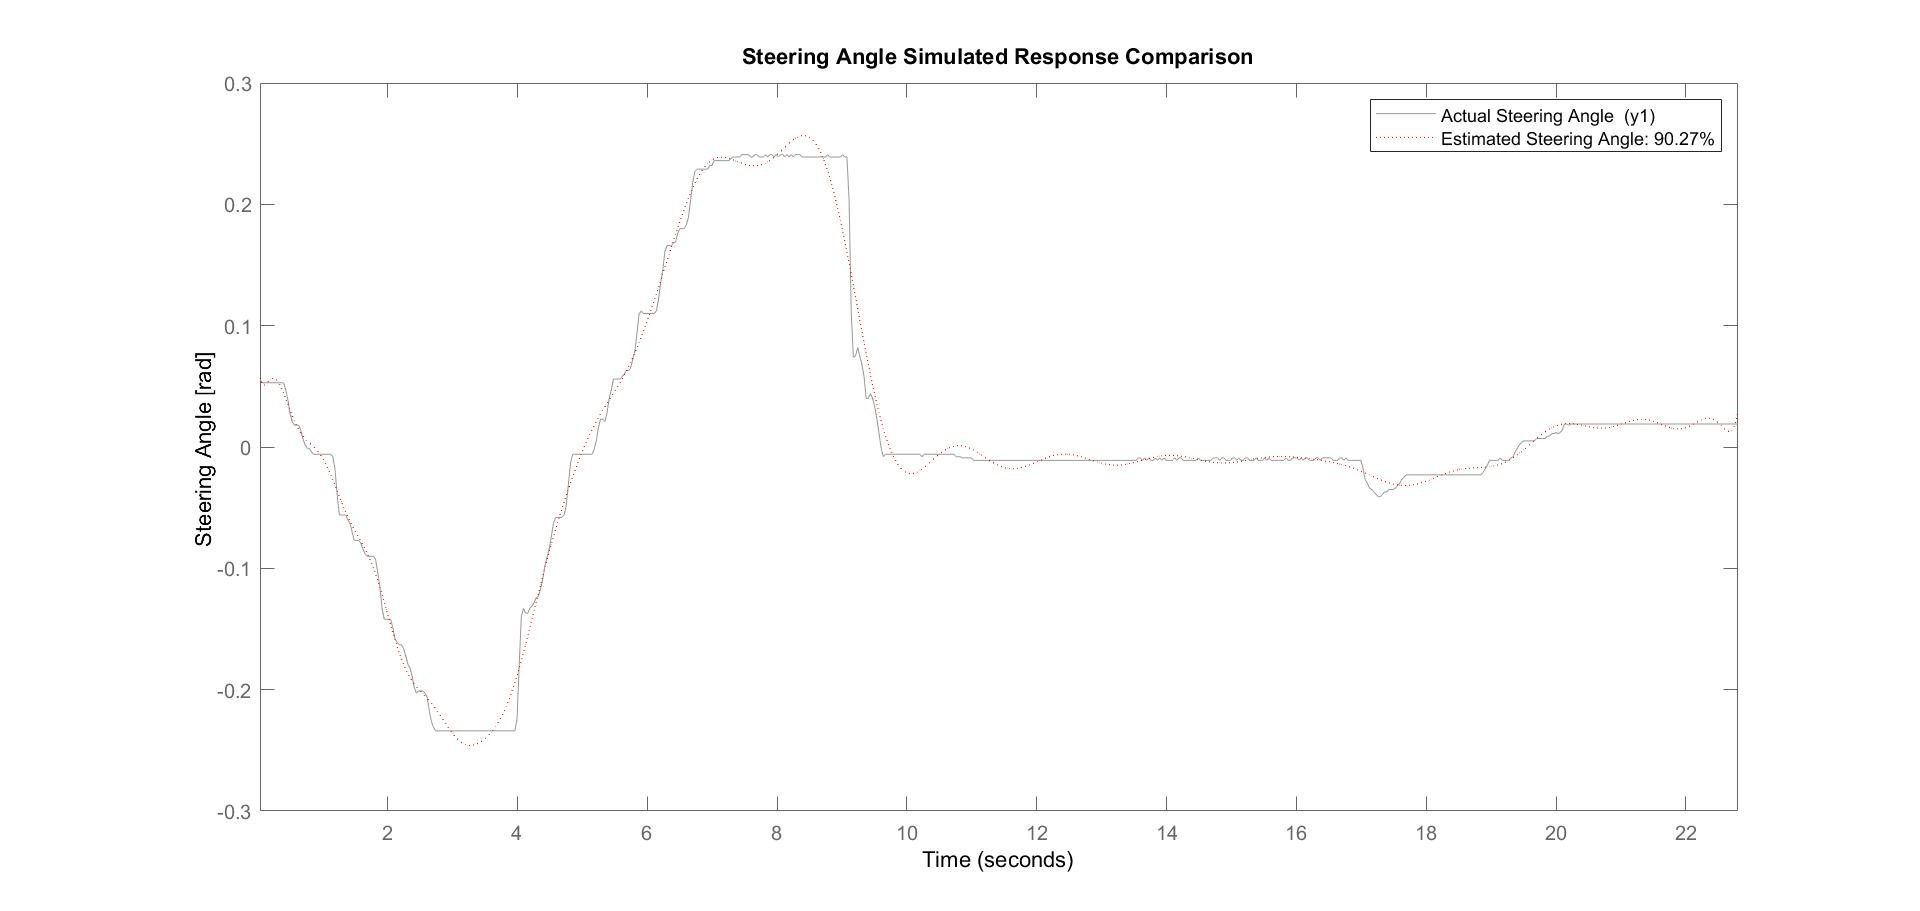
\includegraphics[width=0.48\linewidth]{figs/img/byWireSteeringTransferFunctionModel}}
		{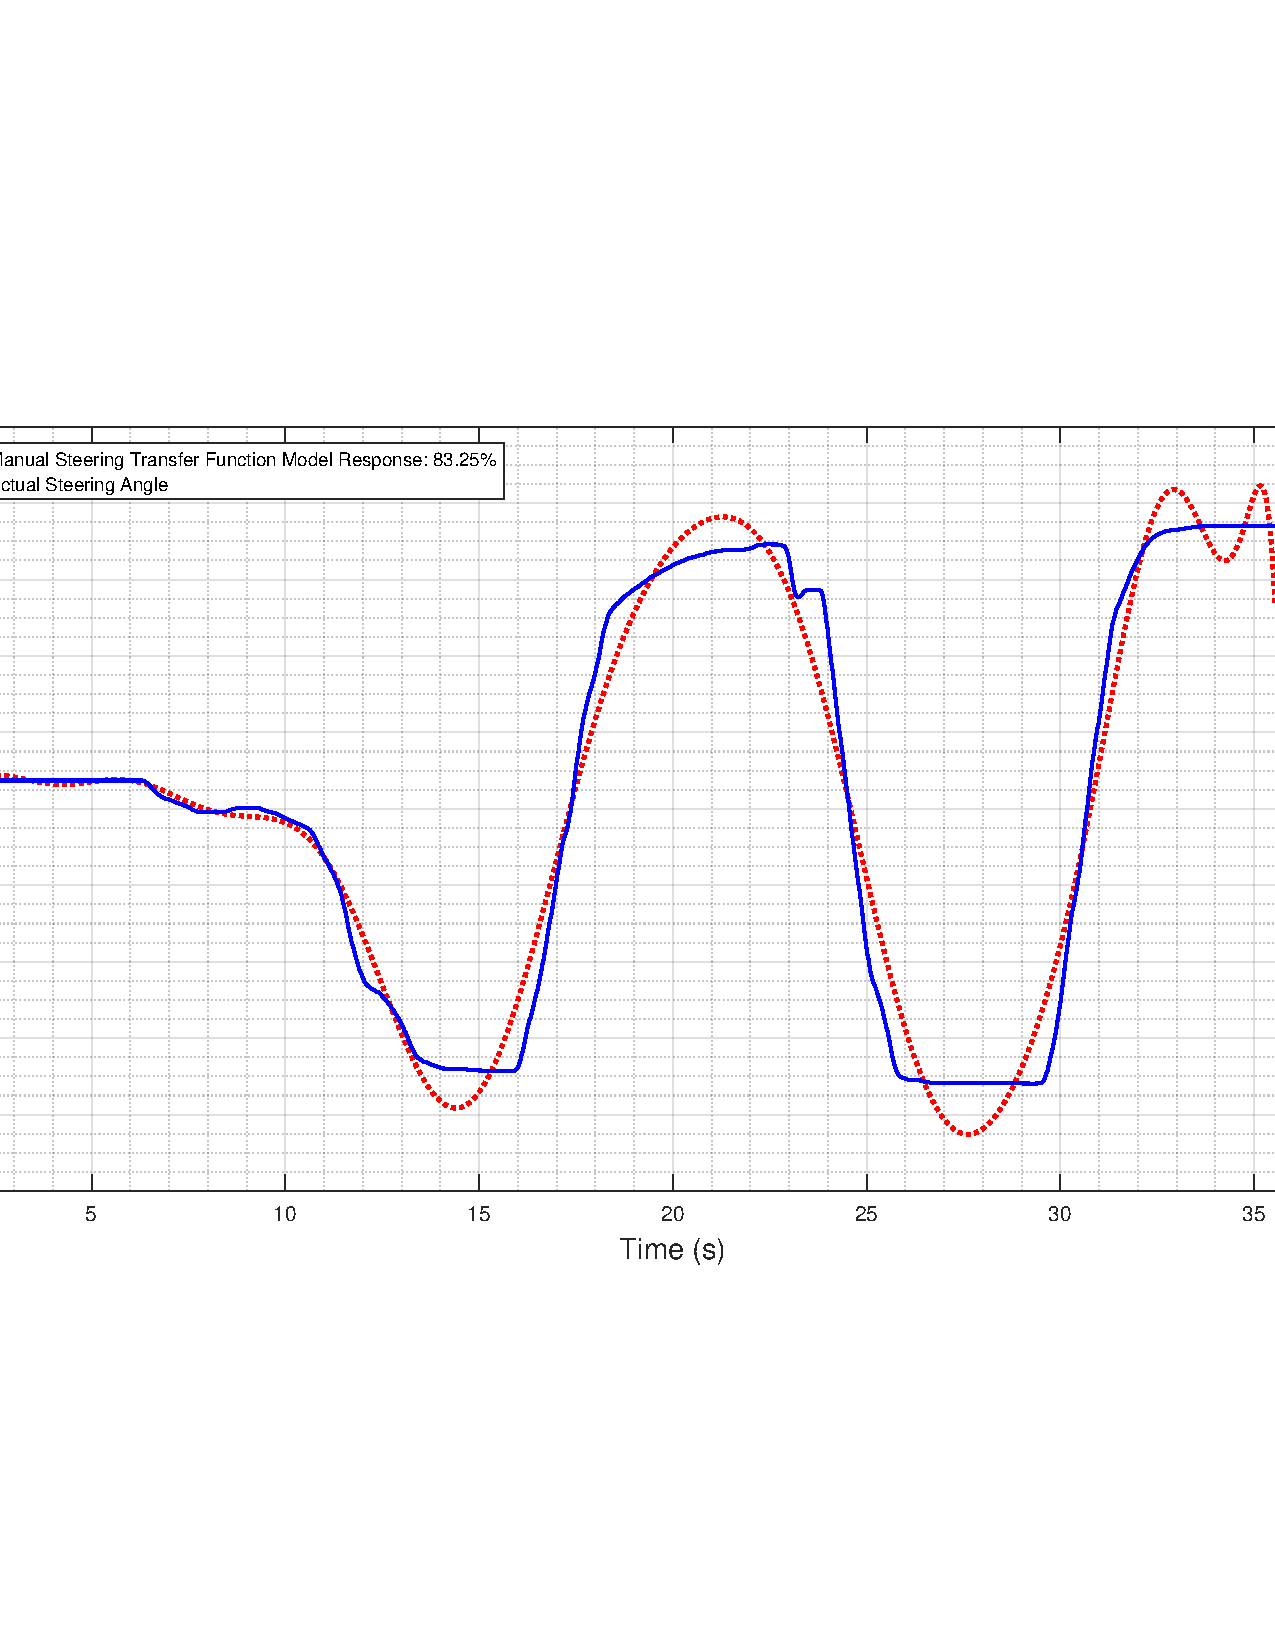
\includegraphics[width=0.48\linewidth]{figs/img/manualSteeringTransferFunctionModel}}
	\caption{Steering System Estimated Steering Angle Comparison}
\end{figure}

\begin{figure}
	\centering
	{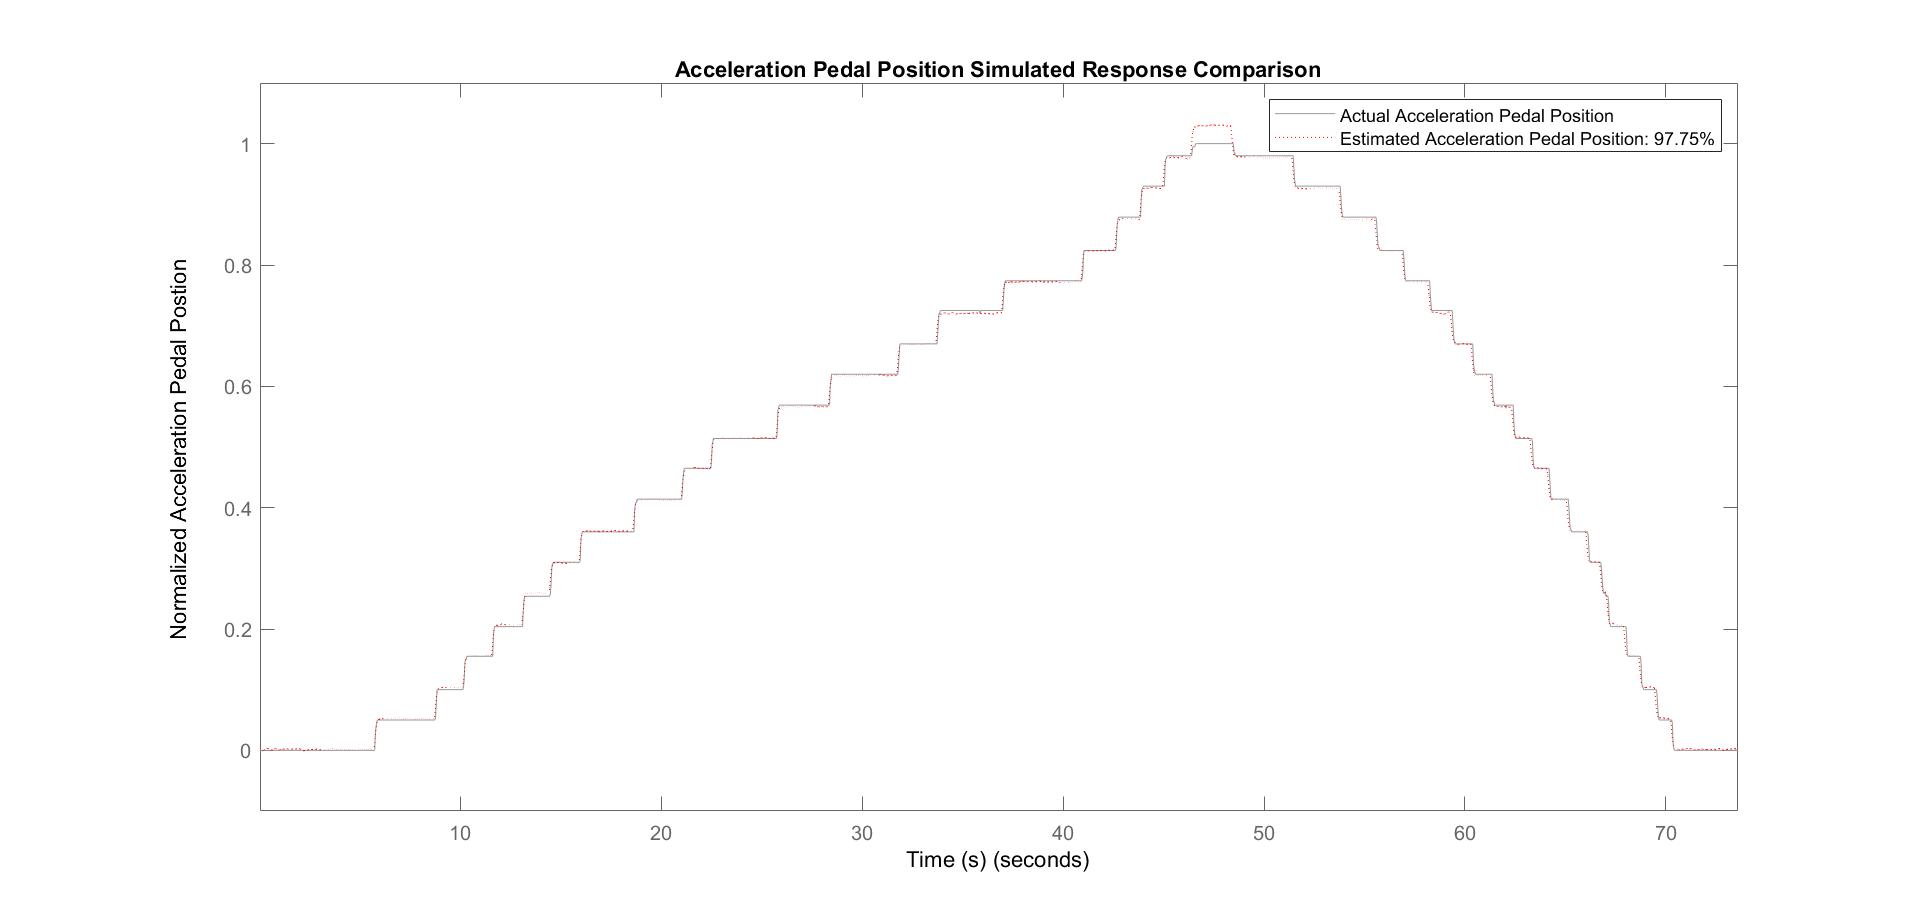
\includegraphics[width=0.48\linewidth]{figs/img/byWireAccelArxModel}}
	{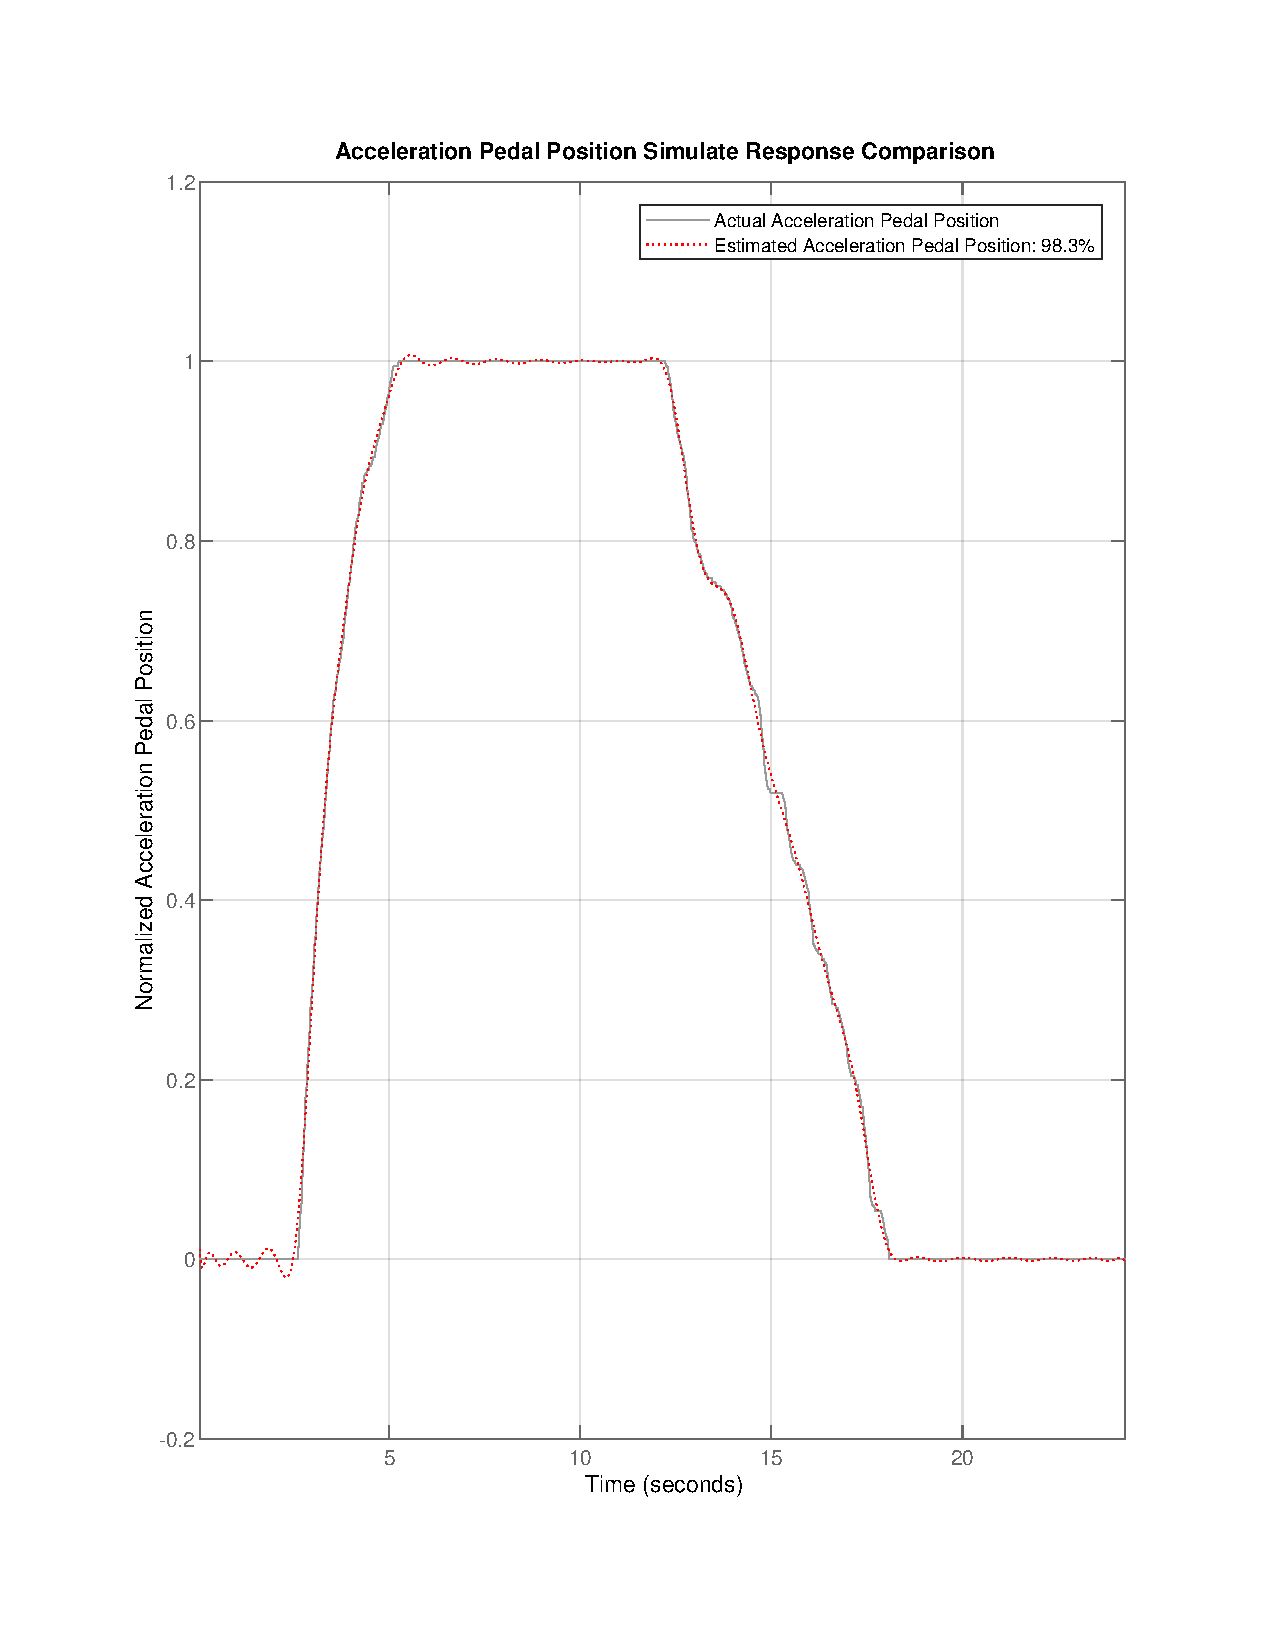
\includegraphics[width=0.48\linewidth]{figs/img/manualAccelTransferFunctionModel}}
	\caption{Acceleration System Estimated Pedal Position Comparison}
\end{figure}

%\vskip -2.5cm
\end{block}

%-----------------------------------------------------------
% NEURAL NETWORK MODELING 
%-----------------------------------------------------------

\begin{block}{Neural Network Modeling}
\vskip -1cm
\begin{itemize}
    \item Used MATLAB's Neural Network Time Series App
    \item Generated models using the Bayesian Regularization Algorithm
    \item Models trained using collected log data  
\end{itemize} 

\begin{figure}
    \centering
		{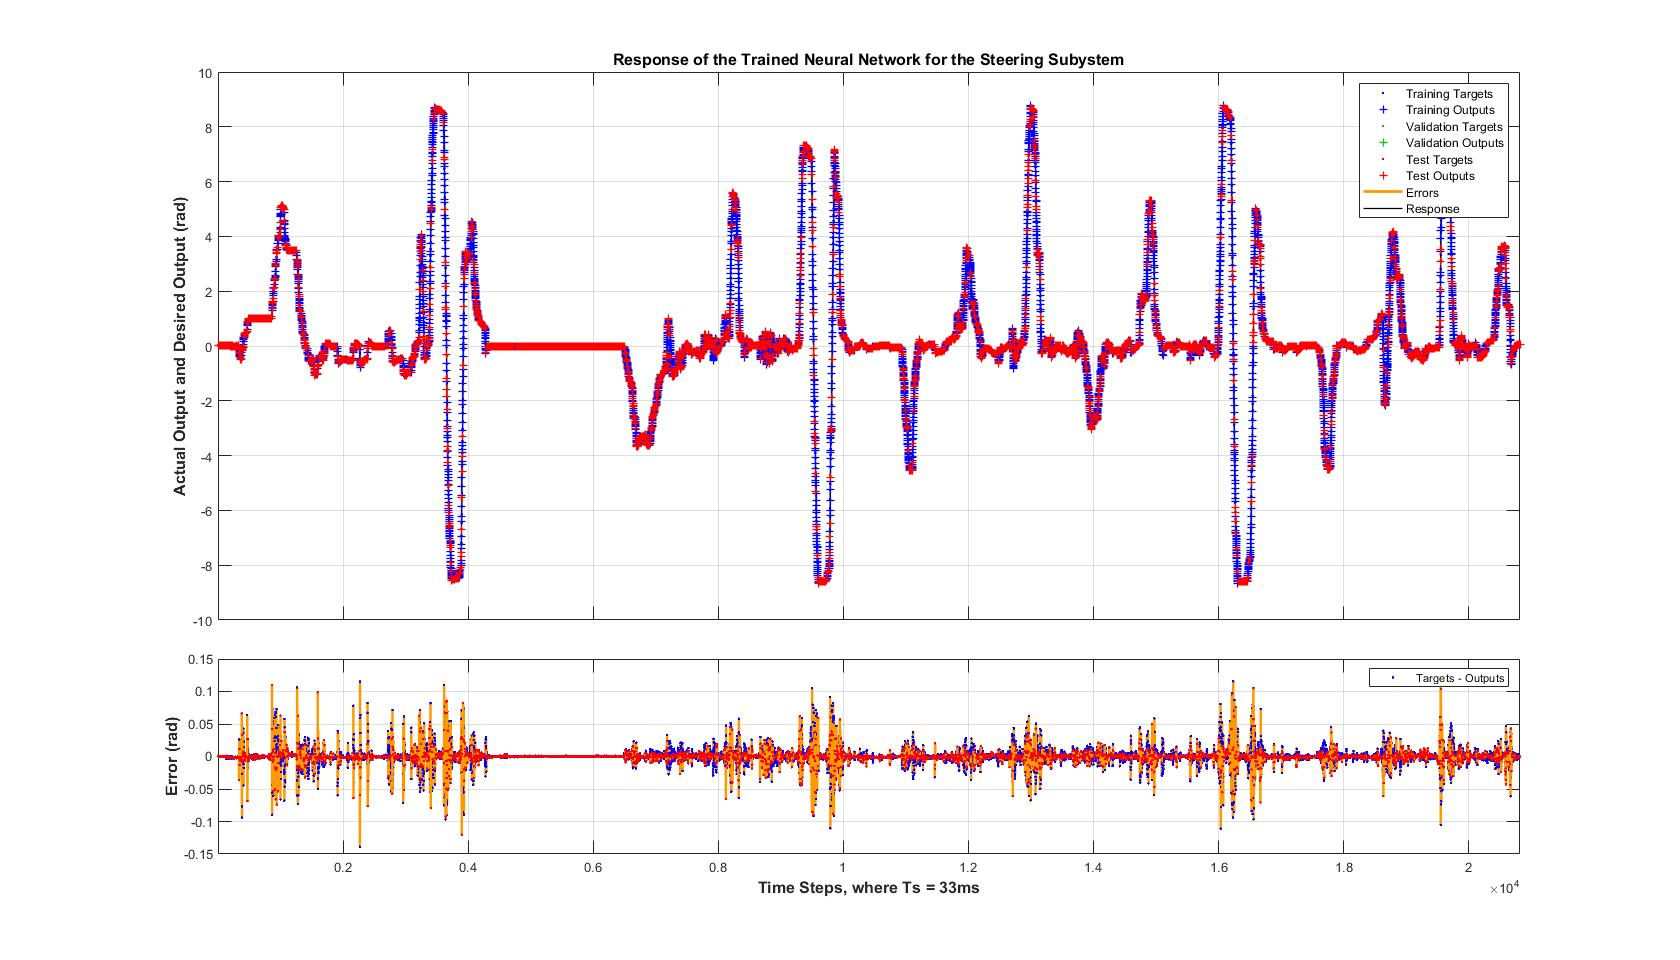
\includegraphics[width=0.48\linewidth]{figs/img/steeringNeuralNetworkTrainedOutput}}
		{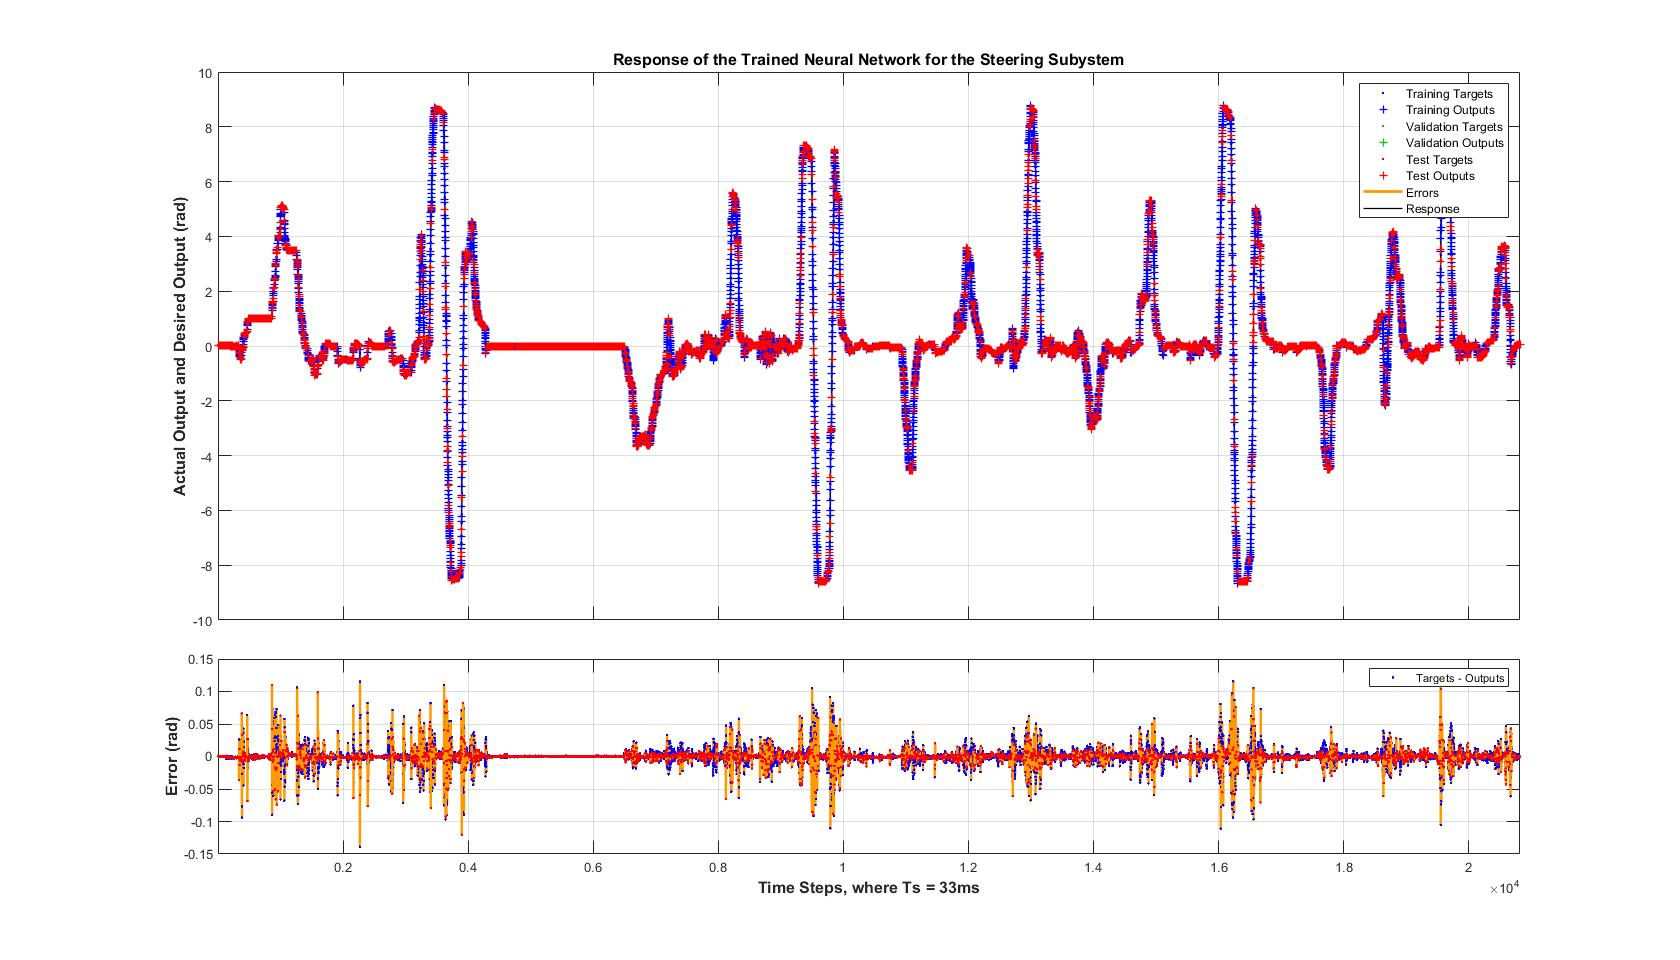
\includegraphics[width=0.48\linewidth]{figs/img/steeringNeuralNetworkTrainedOutput}}
	\caption{Steering System Training Plots}
    \label{fig:SteeringSysNeuralNetwork}
\end{figure}

\begin{figure}
    \centering
		{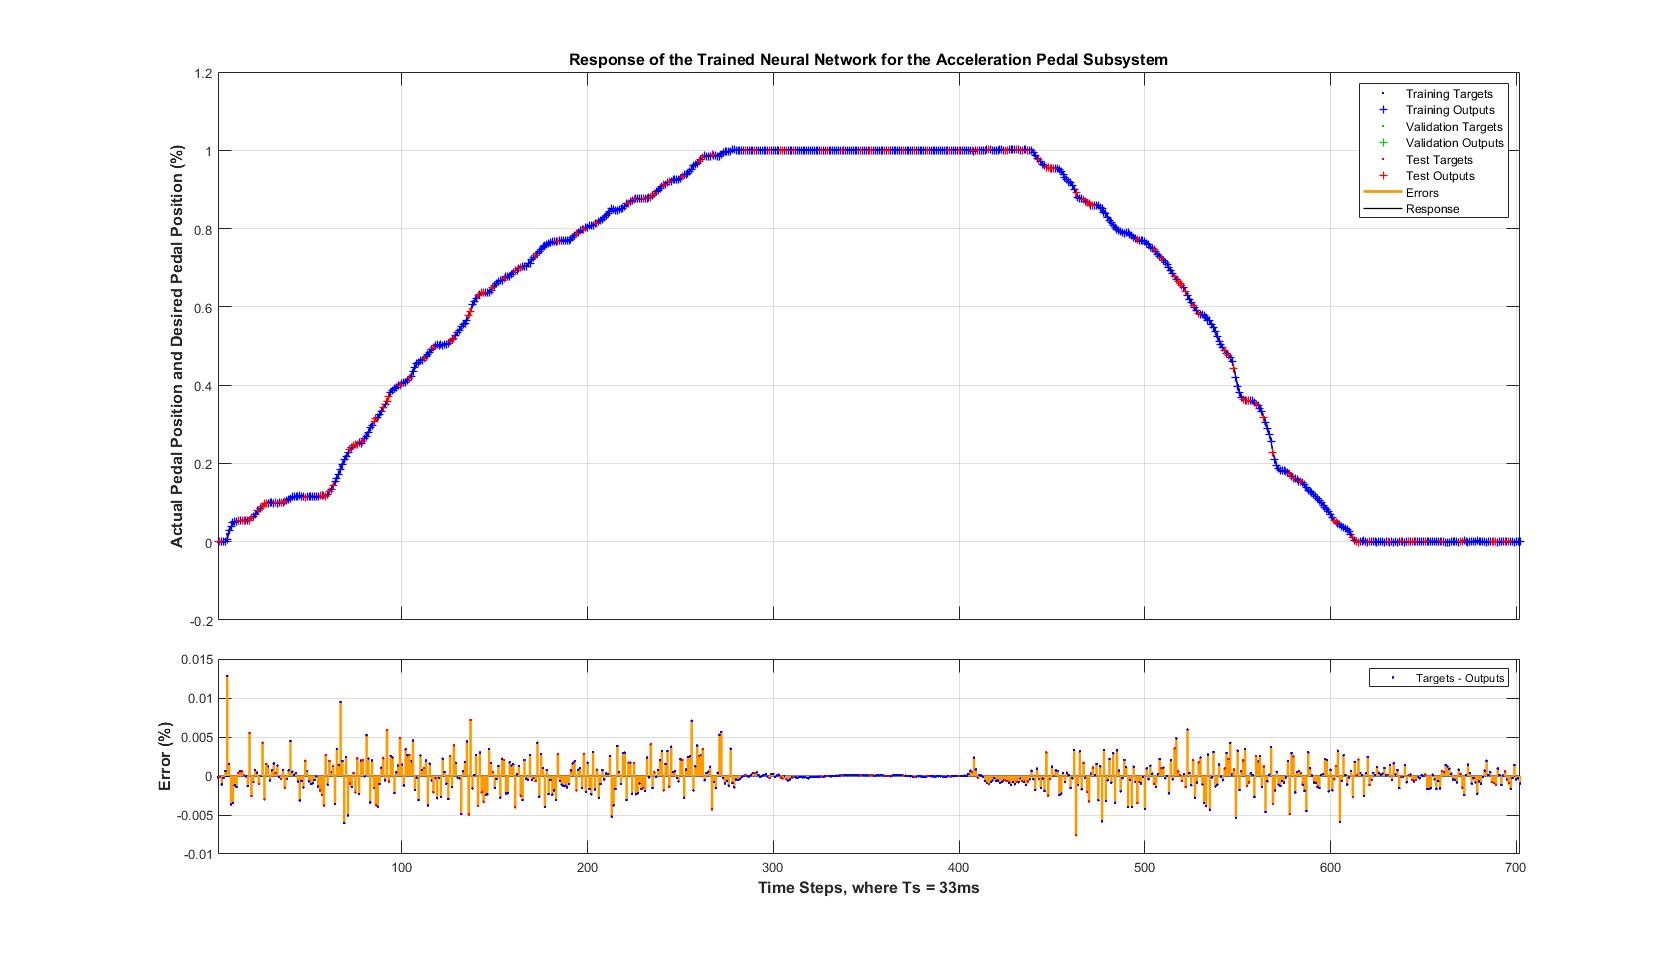
\includegraphics[width=0.48\linewidth]{figs/img/accelNeuralNetworkTrainedOutput}}
		{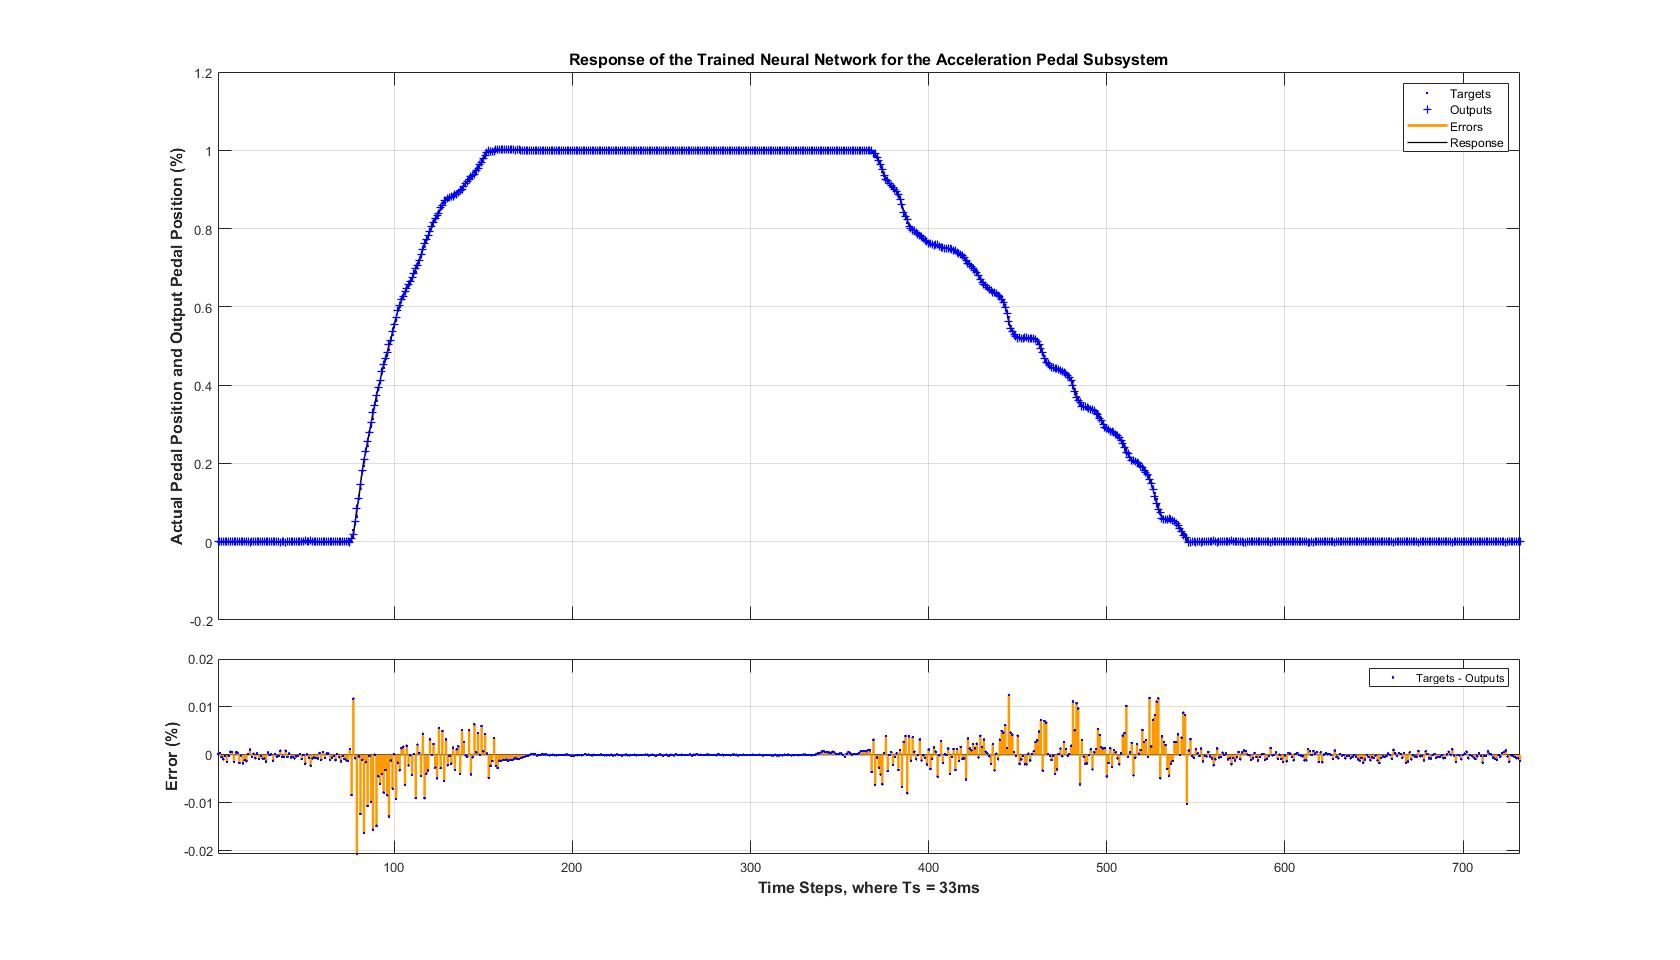
\includegraphics[width=0.48\linewidth]{figs/img/accelNeuralNetworkTrainedOutput2}}
	\caption{Acceleration System Training Plots}
    \label{fig:AccelerationSysNeuralNetwork}
\end{figure}

\begin{figure}
    \centering
		{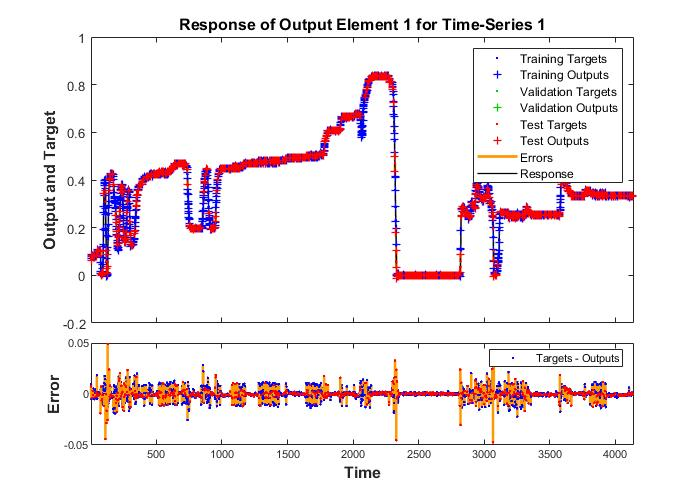
\includegraphics[width=0.48\linewidth]{figs/img/brake_new_neuralNetworkFig}}
		{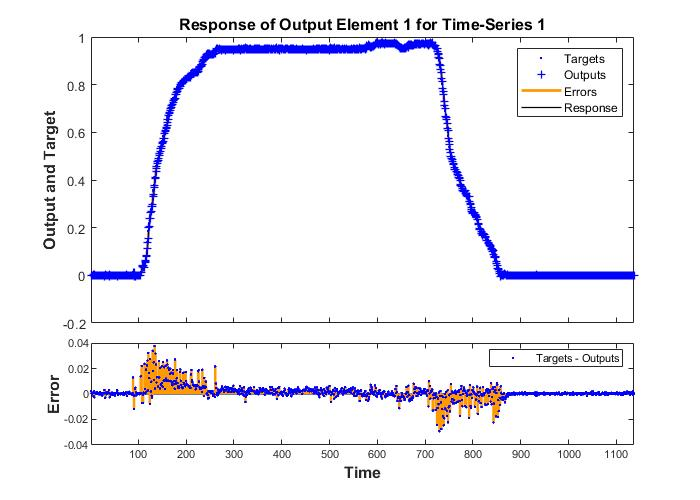
\includegraphics[width=0.48\linewidth]{figs/img/brake_new_neuralNetworkFigLog2Test}}
	\caption{Brake System Training Plots}
    \label{fig:BrakeSysNeuralNetwork}
\end{figure}


%\vskip -2.5cm
\end{block}



\end{column} % End of second column

\begin{column}{\sepwid}\end{column} % Empty spacer column

\begin{column}{\onecolwid} % The third column
%-----------------------------------------------------------
% NEURAL NETWORK ALGORITHM 
%-----------------------------------------------------------

\begin{block}{Neural Network Algorithm}
\vskip -1cm
\begin{itemize}
    %\item Reinforcement learning based approach
    \item Uses neural network based on difference between desired and actual orientation to determine optimal gain
    %\item Unlike LQR, ADP operates only in discrete-time and calculates new gains as the system is running
%    \begin{subequations}
%        \small
%        \begin{align}
%            & some eq = x\\
%            & some eq = y\\
%            & some eq = z
%        \end{align}
%    \label{eq:ADP_EQ}
%    \end{subequations}
\end{itemize} 
%\begin{enumerate}
%    \item Apply input to the system and calculate error e(k) at time k
%    \item Use Euler's method to convert the error model into discrete-time and record data every $\tau \sec$
%    \begin{center}
%        $e_{k+1}=f(e_k)+G(e_k)u_k$
%    \end{center}
%    \item 
%    %\item Minimize the cost function
%    %\begin{center}
%        $J(u)=\sum_{k=0}^{\infty} e_k^TQe_k+u_k^TRu_k$
%    %\end{center}
%    %\item Define value function
%    %\begin{center}
%        $V(e_k)=$
%    %\end{center}    
%    \item Solve for gain, K
%    \begin{center}
%        $K=0.5R^{-1}B^TP$
%    \end{center}
%\end{enumerate}

 \begin{figure}
  \centering
      \tikzset{%
        input neuron/.style={
          circle,
          fill=green!50,
          minimum size=0.7cm
        },
        neuron missing/.style={
          draw=none, 
          scale=1,
          fill=white,
          text height=0.01cm,
          execute at begin node=\color{black}$\vdots$
        },
      }

      \tikzset{%
        hidden neuron/.style={
          circle,
          fill=blue!50,
          minimum size=0.7cm
        },
        neuron missing/.style={
          draw=none, 
          scale=1,
          fill=white,
          text height=0.01cm,
          execute at begin node=\color{black}$\vdots$
        },
      }

      \tikzset{%
        output neuron/.style={
          circle,
          fill=red!50,
          minimum size=0.7cm
        },
        neuron missing/.style={
          draw=none, 
          scale=1,
          fill=white,
          text height=0.01cm,
          execute at begin node=\color{black}$\vdots$
        },
      }      

      \begin{tikzpicture}[x=1.5cm, y=1.5cm]

        \foreach \m/\l [count=\y] in {1,2,missing,3}
        \node [input neuron/.try, neuron \m/.try] (input-\m) at (0,2.5-\y) {};

        \foreach \m [count=\y] in {1,2,3,missing,4}
        \node [hidden neuron/.try, neuron \m/.try ] (hidden-\m) at (2,2.5-\y*1.1) {};

        \foreach \m [count=\y] in {1,missing,2}
        \node [output neuron/.try, neuron \m/.try] (output-\m) at (4,2.5-\y*1.2) {};

        \foreach \l [count=\i] in {1,2,n}
        \draw [<-] (input-\i) -- ++(-1,0)
        node [above, midway] {$\mathbf{e}_{k,\l}$};

        \foreach \l [count=\i] in {1,2,3,\mbox{$\bar{n}$}}
        \node [above] at (hidden-\i.north) {$\sigma_{\l}$};

        \foreach \l [count=\i] in {1,m}
        \draw [->] (output-\i) -- ++(1,0)
        node [above, midway] {$\hat{u}_{a,k}^{(\l)}$};

        \foreach \i in {1,...,3}
        \foreach \j in {1,...,4}
        \draw [->] (input-\i) -- (hidden-\j);

        \foreach \i in {1,...,4}
        \foreach \j in {1,2}
        \draw [->] (hidden-\i) -- (output-\j);


        
        \foreach \l [count=\x from 0] in {Input, Hidden, Ouput}
        \node [align=center, above] at (\x*2,1.9) {\l \\ layer};

        \node [align=center, below] at (3,-2.5) {Weight \\ $\mathbf{W}_a$};
        \draw[->,ultra thick](3,-2.5) -- (3,1.6);
        
      \end{tikzpicture}
  \caption{Actor neural network structure for approximating control input.}
  \label{fig:nnActor}
\end{figure}



\vskip 1.5cm
%(1) t = kτ where τ is given
%(2)Advance the system by applying determined inputs to the system and measure system states
%(3)Calculate state error as e[k] = xref[k] − x[k], save state error
%(4) If t 6= T, increment k and start at (1)
%(5) If t = T, update K using collected error data
%(5a)Use error states since last update of K as inputs to the neural network
%(5b)Recursively determine wc values for each of the instances
%(5c)Approximate new wc value using regression analysis of the individually calculated wc values
%(6)Calculate new K using wc values
%(7) Increment k and start at (1)


\vskip -2.5cm
\end{block}
%-----------------------------------------------------------
% Subsystem Block Diagram
%-----------------------------------------------------------


%-----------------------------------------------------------
% SIMULATION RESULTS
%-----------------------------------------------------------

\end{column} % End of third column

\begin{column}{\sepwid}\end{column}

\begin{column}{\onecolwid} % The fourth column

%-----------------------------------------------------------
% EXPERIMENTAL RESULTS
%-----------------------------------------------------------

\begin{block}{Experimental Results}
\vskip -1cm
\begin{itemize}
    \item Preliminary model testing conducted before sending models to AutonomouStuff 
    \item Official testing conducted at AutonomouStuff using...
\end{itemize}
\begin{figure}
    \centering
    \fcolorbox{gray!10}{gray!10}{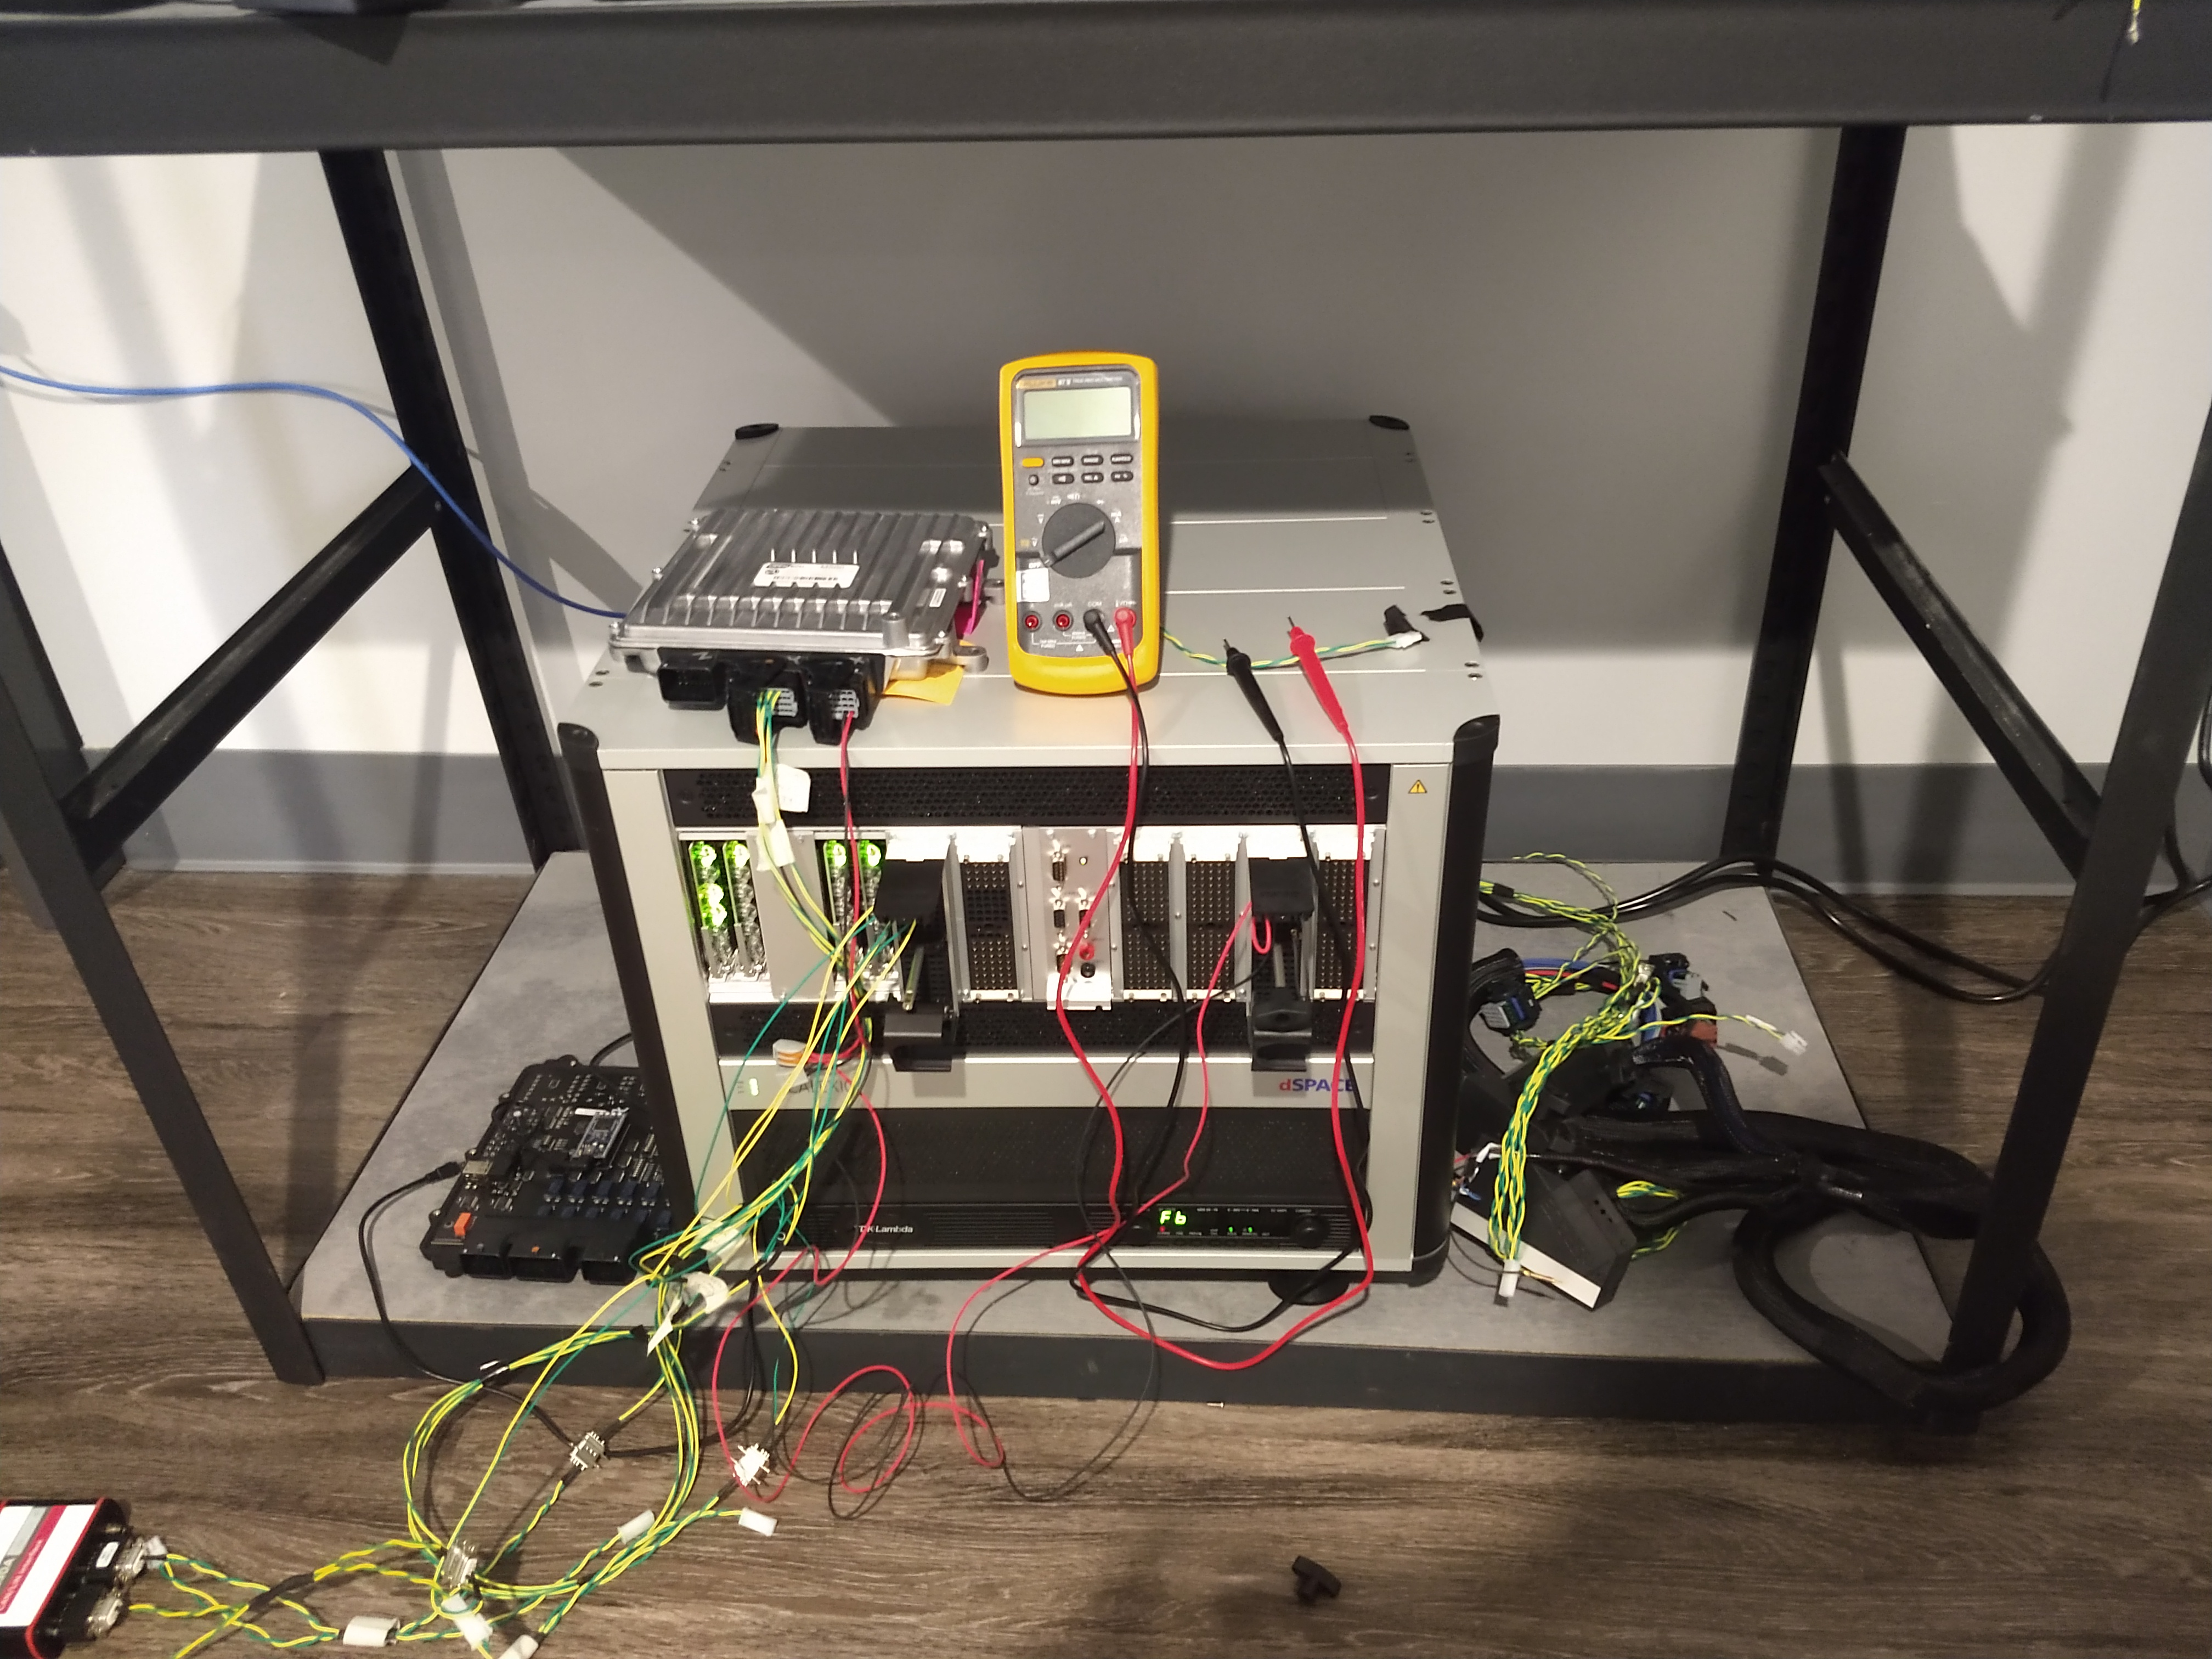
\includegraphics[height=.15\textheight,width=.9\textwidth,keepaspectratio=true]{figs/img/picturesVisitToAStuff/hilBenchAstuff.jpg}}
    \caption{Experimental Setup}
    \label{fig:Setup}
\end{figure}

\begin{figure}
    \centering
    \subfigure[][]{
    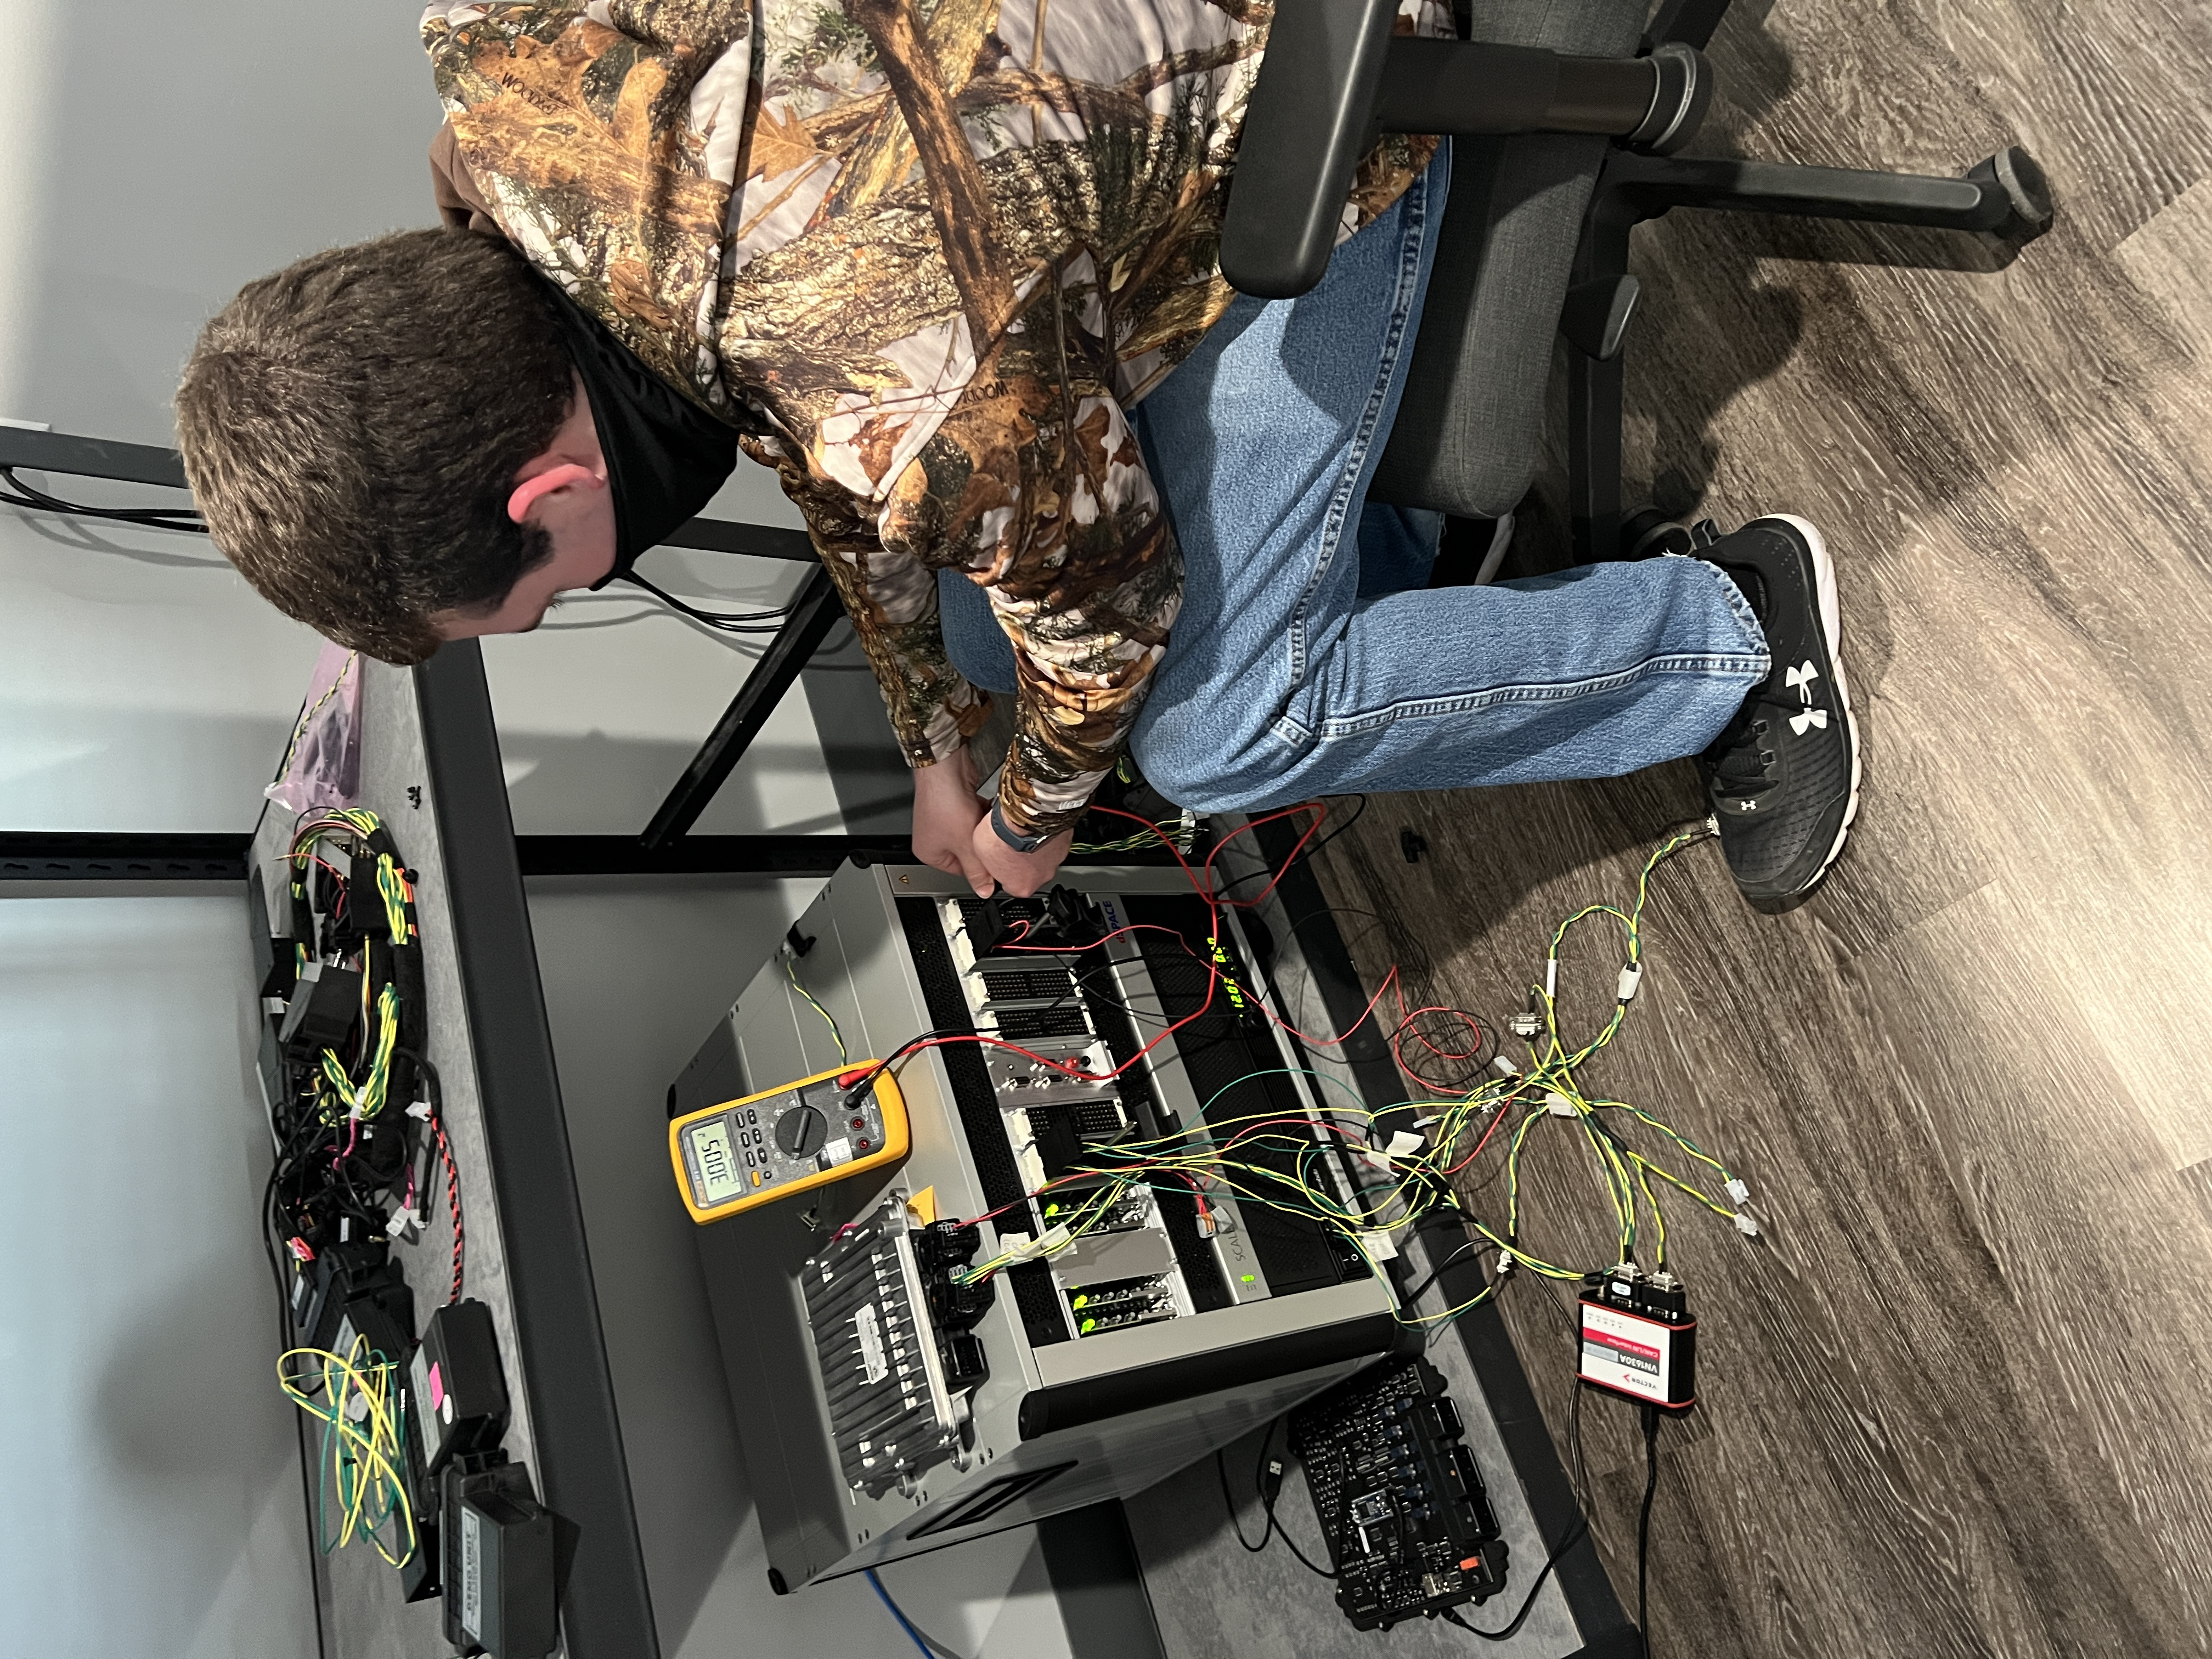
\includegraphics[width=.46\textwidth,keepaspectratio=true]{figs/img/picturesVisitToAStuff/aStuffVisit2Nick}
    }
    \subfigure[][]{
    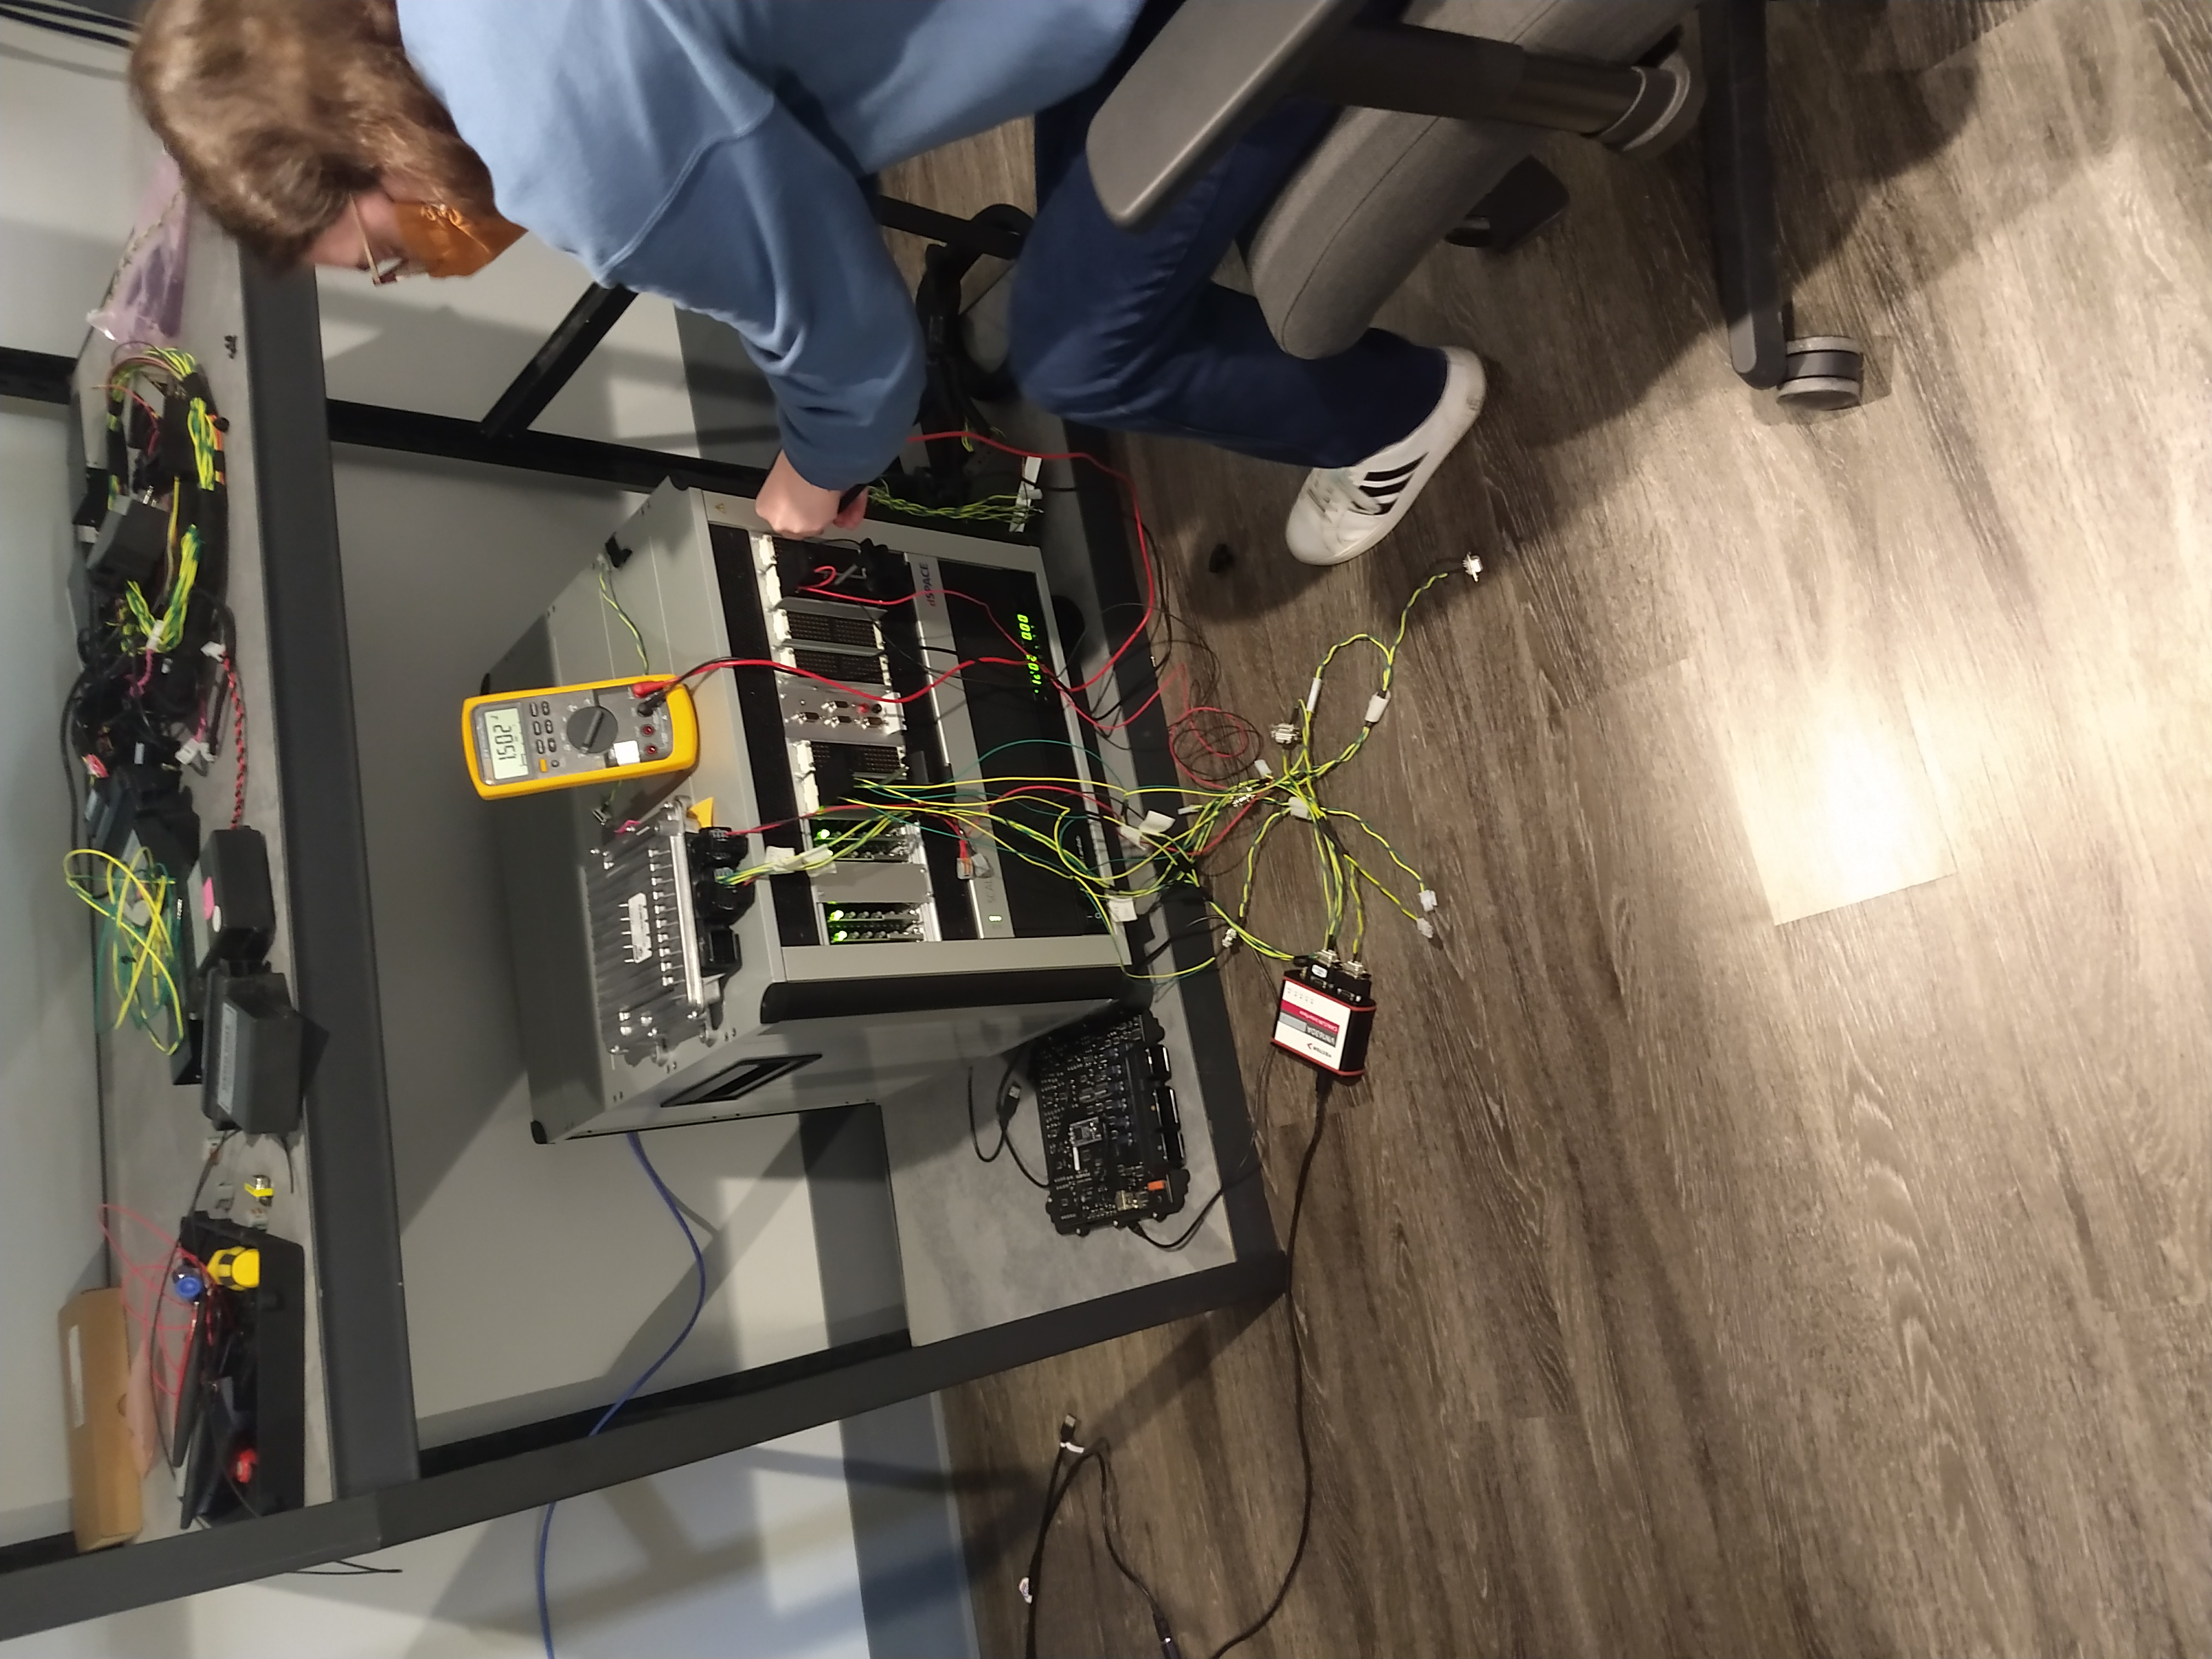
\includegraphics[width=.46\textwidth,keepaspectratio=true]{figs/img/picturesVisitToAStuff/hilMeasurementHannah}
    }
    \caption{Verifying voltage measurements on the HIL Bench}
\end{figure}

\vskip -.5cm

\vskip -2cm
\end{block}


%-----------------------------------------------------------
% Conclusion and Future Work
%-----------------------------------------------------------

\begin{alertblock}{Conclusion and Future Work}
\begin{itemize}
    \item Using Neural Networks produced more accurate models than System Identification 
   % \item PI controller greatly reduces steady-state error, however increases overshoot and settling time
    \vskip .75cm
    \item Test models using Hardware-in-the-Loop
    \item Create new vehicle controllers
\end{itemize}


\end{alertblock}

\end{column} % End of the fourth column

\end{columns} % End of all the columns in the poster

\end{frame} % End of the enclosing frame

\end{document}

%%% Local Variables:
%%% mode: latex
%%% TeX-master: t
%%% End:
